% Clean CV/Resume Template, by Bennet B <dev@bennet.cc>
% CC0, Public-Domain
%
% Permission is hereby granted, free of charge, to any person obtaining a copy
% of this template and associated files (the "Template"), to deal
% in the Template without restriction, including without limitation the rights
% to use, copy, modify, merge, publish, distribute, sublicense, and/or sell
% copies of the Template, and to permit persons to whom the Template is
% furnished to do so, subject to the following conditions:
%
% The above copyright notice and this permission notice shall be included in all
% copies or substantial portions of the Template.
%
% THE TEMPLATE IS PROVIDED "AS IS", WITHOUT WARRANTY OF ANY KIND, EXPRESS OR
% IMPLIED, INCLUDING BUT NOT LIMITED TO THE WARRANTIES OF MERCHANTABILITY,
% FITNESS FOR A PARTICULAR PURPOSE AND NONINFRINGEMENT. IN NO EVENT SHALL THE
% AUTHORS OR COPYRIGHT HOLDERS BE LIABLE FOR ANY CLAIM, DAMAGES OR OTHER
% LIABILITY, WHETHER IN AN ACTION OF CONTRACT, TORT OR OTHERWISE, ARISING FROM,
% OUT OF OR IN CONNECTION WITH THE TEMPLATE OR THE USE OR OTHER DEALINGS IN THE
% TEMPLATE.
%
% based on Modern CV by Habib Semouma
% https://www.overleaf.com/latex/templates/modern-cv-slash-resume-template/vjrqdkpjckwj
%
%
\documentclass[UTF8]{article}
\usepackage{wallpaper}
\usepackage[UTF8,fontset=none]{ctex}
\usepackage{xeCJK}
\setCJKmainfont{PingFang SC}
\setCJKsansfont{PingFang SC}
\setmainfont{PingFang SC}
\setsansfont{PingFang SC}
\usepackage{geometry}
\usepackage{enumitem}
\usepackage{tikz}
\usepackage[
    unicode=true,
    bookmarks=true,
    bookmarksnumbered=false,
    bookmarksopen=true,
    bookmarksopenlevel=1,
    breaklinks=false,
    pdfborder={0 0 0},
    backref=false,
    colorlinks=false
    ]{hyperref}
\usepackage{lastpage}
\usepackage{hyphenat}
\usepackage{hyphsubst}
\usepackage{tabularx}
\usepackage{moresize}
\usepackage[document]{ragged2e}
% \usepackage{parskip}

\usepackage[scaled]{helvet}
\usepackage{fontawesome5}
\usepackage[defaultfam,tabular,oldstyle]{montserrat}
\usepackage[T1]{fontenc}
\renewcommand*\oldstylenums[1]{{\fontfamily{Montserrat-TOsF}\selectfont #1}}

\usepackage{titlesec}
\usepackage{xcolor}
\usepackage{tikz}
\usepackage{pgfornament}
\setlength{\parindent}{0pt}
\titleformat{\section}{\normalfont}{}{0pt}{}

\renewcommand{\arraystretch}{1.15}

\setlength\fboxrule{0pt}
\setlength\fboxsep{6pt}
% \setlength{\parskip}{.5\baselineskip plus 2pt}
% \renewcommand{\baselinestretch}{1.1}

\titlespacing{\section}{0pt}{0.8ex plus .1ex minus .1ex}{0.4ex}
%%%%%%%%%%%%%%%%%
% New Command
\newcommand{\starrating}[1]{%
    \makebox[2cm][l]{\raisebox{-0.5ex}{\foreach \x in {1,...,#1}{\textcolor{yellow}{\faStar}\hspace{0.2em}}}}
}

% 定义更大的bullet点
\renewcommand{\labelitemi}{\large$\bullet$}

%%%%%%%%%%%%%%%%%%%
\newcolumntype{Y}{>{\RaggedRight\arraybackslash}X}

% Change PDF Meta Info here
\hypersetup{
    pdftitle={郑鑫裕 - CV - 中文},
    pdfauthor={郑鑫裕},
    pdfsubject={CV}
}

% Paper size
\geometry{
    a4paper,
    left=1.2cm,
    right=1.2cm,
    top=1.0cm,
    bottom=1.0cm,
    nohead,
    nomarginpar
}

% Background Color of the Sidebar Column
% \definecolor{sidebg}{cmyk}{1, 0.02, 0, 0.56}
\definecolor{sidebg}{cmyk}{0.2, 0.05, 0.15, 0}
% \definecolor{sidebg}{rgb}{0.8, 0.8, 0.9}
% Background Color of the Main Column
\definecolor{mainbg}{cmyk}{0, 0, 0.07, 0.04}

% Text Color of the Main Column
\definecolor{maintext}{cmyk}{1, 0.02, 0, 0.8}
% Text Color of the Sidebar Column
% \definecolor{sidetext}{cmyk}{0, 0, 0.07, 0.04}
\definecolor{sidetext}{cmyk}{1, 0.02, 0.5, 0.8}
\pagecolor{white}

\begin{document}
\setlength{\topskip}{0pt}\setlength{\footskip}{0pt}%
\color{maintext}
\pagestyle{empty}

\begin{minipage}[t]{0.83\textwidth}
    {\bfseries\fontsize{24}{28}\selectfont 郑鑫裕} \\
    \vspace{0.2em}
    {\large 生成式AI / 计算机视觉 / 多模态算法或研究实习生} \\
    \vspace{0.45em}
    {\small
    \faPhone{} 150 7938 0535 \quad
    \faEnvelope{} \href{mailto:3193603347@qq.com}{3193603347@qq.com}
    } \\
    {\small
    \faMapMarker{} 陕西省西安市西咸新区西安交通大学创新港校区惠园
    } \\
    \vspace{0.35em}
    {\small \faTools{} \textbf{技能}：Python $\cdot$ C/C++ $\cdot$ PyTorch $\cdot$ OpenCV $\cdot$ 扩散模型 $\cdot$ LoRA微调 $\cdot$ Transformer $\cdot$ YOLO $\cdot$ ComfyUI $\cdot$ } \\
    {\small \hspace*{4em} Git $\cdot$ Linux(Arch/Ubuntu) $\cdot$ Emacs} \\
    {\small \faLanguage{} \textbf{语言}：英语 CET6 \quad $\vert$ \quad 法语 DELF C1} \\
\end{minipage}
% \hfill
\begin{minipage}[t]{0.17\textwidth}

    \begin{center}
        \vspace{-1.5em}
        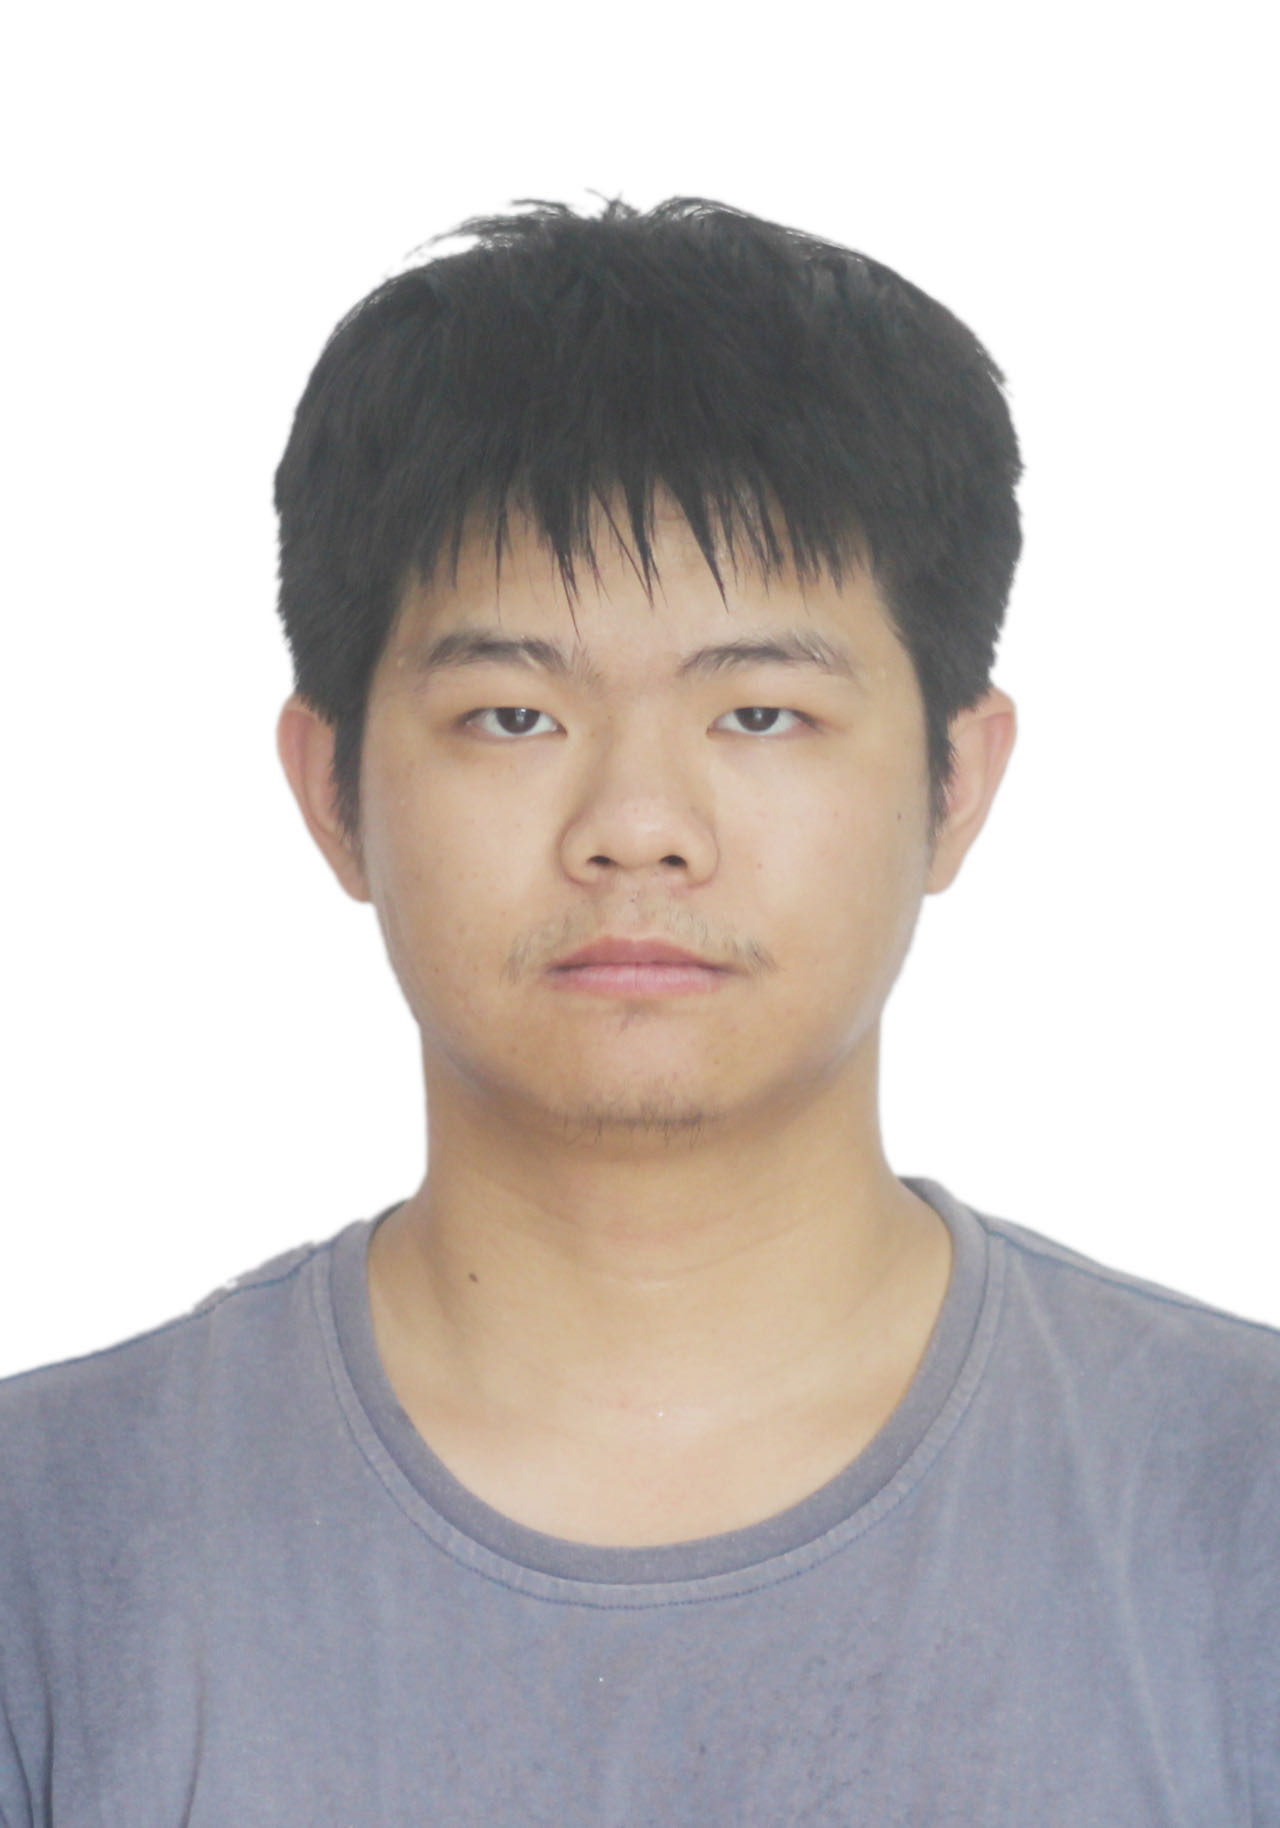
\includegraphics[width=3.0cm]{cv_picture.jpg}
    \end{center}
\end{minipage}

\vspace{0.35em}
{\small \faInfoCircle{} \textbf{简介}：具备生成式AI与计算机视觉相关项目经验，熟悉从数据处理、模型训练到效果优化的完整流程，能够从零实现扩散模型训练与推理框架，并具备多卡机器训练经验。拥有中法双学位与海外实习经历，能够在跨文化环境中高效协作。关注扩散模型与图像、视频生成及压缩方向，兼顾研究探索与业务落地。}

\vspace{0.35em}
\hrule
\vspace{0.35em}

%%%%%%%%%%%%%%%%%%%%%%%%%%%%%%%%%%%%%%%%%%%%%%%%%%%%%%%%%%%
        % EDUCATION
% \phantomsection{}
\addcontentsline{toc}{section}{教育背景}
\section*{\bfseries\large 教育背景}
\begin{tabularx}{\linewidth}{X r}
    \normalsize \textbf{西安交通大学} & 2025.09 - 至今 \\
\end{tabularx}
\begin{itemize}[leftmargin=1.6em, itemsep=0em, topsep=0.05em, parsep=0pt]
    \item 硕士在读，西安交通大学人机所，人工智能专业；获一等学业奖学金，推免录取
    \item 研究方向：基于\strong{扩散模型}或\strong{自回归模型}的\strong{生成式图像与视频压缩}
\end{itemize}

\begin{tabularx}{\linewidth}{X r}
    \normalsize \textbf{法国中央理工大学（双学位）} & 2023.09 - 2025.07 \\
\end{tabularx}
\begin{itemize}[leftmargin=1.6em, itemsep=0em, topsep=0.05em, parsep=0pt]
    \item 通用工程师学位；担任\strong{国际学生联合会主席、中国学生联合会会计、学生会国际生代表}
\end{itemize}

\begin{tabularx}{\linewidth}{X r}
    \normalsize \textbf{西安交通大学} & 2021.09 - 2025.07 \\
\end{tabularx}
\begin{itemize}[leftmargin=1.6em, itemsep=0em, topsep=0.05em, parsep=0pt]
    \item 本科，人工智能；成绩 89.68/100，专业前 30\%
    \item 核心课程：深度学习、计算机视觉、强化学习、机器学习、模式识别、嵌入式系统
    \item 获中外联合培养机会，领 CSC 奖学金，赴法完成大三大四学业
\end{itemize}

\vspace{0.15em}
\hrule
\vspace{0.2em}

%%%%%%%%%%%%%%%%%%%%%%%%%%%%%%%%%%%%%%%%%%%%%%%%%%%%%%%%%%
        % WORK EXPERIENCE
% \phantomsection{}
\addcontentsline{toc}{section}{专业经历}
\section*{\bfseries\large 专业经历}

\begin{tabularx}{\linewidth}{X r}
    \normalsize \textbf{北京零一智能科技有限公司 算法实习生} & 2025.11 - 2026.02 \\
\end{tabularx}
\begin{itemize}[leftmargin=1.6em, itemsep=0em, topsep=0.05em, parsep=0pt]
    \item 基于 EasyAnimate（Video-DiT）,采用 CatV2TON 方案，结合 LiON-LoRA 方法微调，通过清洗企业闭源数据并优化训练策略，解决基于多图的 VideoTryOn 模型中的动作、服装细节一致性，提升模型稳定性，产出可用于生产的图像换装模型。
    \item 基于 ComfyUI 搭建端到端视频换装流程。
    \item 使用 Nano Banana 与 ChatGPT 设计复杂材质衣物镂空图生成提示词，将生成成功率提升至 99\% 以上。
\end{itemize}

\begin{tabularx}{\linewidth}{X r}
    \normalsize \textbf{Groupe Bouygues 研究性实习} & 2024.05 - 2024.08 \\
\end{tabularx}
\begin{itemize}[leftmargin=1.6em, itemsep=0em, topsep=0.05em, parsep=0pt]
    \item 开发基于 AI 视频理解的工地智能安全头盔系统，结合实地调研识别 8 类主要风险场景。
    \item 参考 ST-GCN 与 SkateFormer 等骨架序列建模方法，采用 YOLOv5s-pose 提取人体关键点，并结合 Transformer 架构对跨帧时序信息与关键点空间关系进行联合建模，在企业数据集上完成训练，风险场景分类准确率达到 94\%。
    \item 基于 Arduino 和 ESP32-CAM 平台实现硬件原型，集成边缘计算模块，用于工地安全智能监控。
\end{itemize}

\begin{tabularx}{\linewidth}{X r}
    \normalsize \textbf{LamCube 研究性实习} & 2024.02 - 2024.03 \\
\end{tabularx}
\begin{itemize}[leftmargin=1.6em, itemsep=0em, topsep=0.05em, parsep=0pt]
    \item 围绕建筑裂缝智能检测开展研究，调研并分析 50 余篇建筑及工业领域 AI 检测相关文献；采用 Deeplabv3+ 语义分割方案，并结合传统图像处理方法进行优化，在实验室数据集上完成训练，最终实现 IoU 为 0.84。
    \item 围绕自动驾驶小车原型开展研究，基于 YOLO 实现实时车道线检测、行人检测及车标检测，并结合 Arduino 与嵌入式 GPU 平台完成系统搭建。
\end{itemize}
\vspace{0.15em}
\hrule
\vspace{0.2em}
\addcontentsline{toc}{section}{科研经历}
\section*{\bfseries\large 科研经历}

\begin{tabularx}{\linewidth}{X r}
    \normalsize \textbf{基于矢量量化与生成模型的图像压缩方法研究} & 2024.09 - 2025.06 \\
\end{tabularx}
\begin{itemize}[leftmargin=1.6em, itemsep=0em, topsep=0.05em, parsep=0pt]
    \item 围绕矢量量化器开展研究，对 VQVAE、RVQ、FSQ 等量化编码器及基于 MaskGIT 与 MAE 的 ROI 区域图像编解码进行调研。
    \item 结合 Stable Diffusion、HyperPrior 熵编码与传统图像处理方法设计压缩方案，实现 500 倍以上压缩比（0.002 bpp）。
\end{itemize}

% \begin{tabularx}{\linewidth}{X r}
%     \large \textbf{腾飞杯创新竞赛} &  May 2023 \\
% \end{tabularx}
% {构建ARIMA时间序列预测模型，分析疾病时间序列数据与新冠病毒发病率的关联性,模型拟合度$R^2$达到0.89} \\[0.6em]

% \begin{tabularx}{\linewidth}{X r}
%     \large \textbf{数学建模比赛} &  Aug. 2022 \\
% \end{tabularx}
% {使用Scrapy框架爬取10万+房源数据,构建深度学习房价预测系统,预测准确率92.1\%。} \\[0.6em]
\end{document}
